\documentclass[12pt,letter]{article}
\usepackage{../downey_format}


\begin{document}
	
	% set the section number, along with figure and equation numbers
	\setcounter{section}{0}	
	\setcounter{figure}{\thesection}   
	\renewcommand\thefigure{\thesection.\arabic{figure}}
	\setcounter{equation}{\thesection}   
	\renewcommand\theequation{\thesection.\arabic{equation}}


\section{Basic Concepts in Machine Learning}

\begin{figure}[bp!]
    \centering
    \includegraphics[width=\linewidth]{../figures/AI-vs-ML-vs-Deep-Learning}
    \caption{Overlap between the fields of Artificial Intelligence (AI), Data science (DS), and the core engineering disciplines of Civil, Mechanical, Electrical, and Chemical Engineering.}
    \label{fig:AI-vs-ML-vs-Deep-Learning}
\end{figure}

Machine Learning (ML) is a method of data analysis that automates analytical model building. ML is closely coupled to data science, as shown in figure~\ref{fig:AI-vs-ML-vs-Deep-Learning}, which is a multidisciplinary field that utilizes scientific methods, processes, algorithms, and systems to extract knowledge and insights from structured and unstructured data. It is based on the idea that systems can learn from data, identify patterns, and make decisions with minimal human intervention. This section introduces some foundational concepts in machine learning and its applications.

\begin{itemize}
    \item \textbf{ML is not creating robots}: A common misconception is that machine learning is about building robots. In reality, ML focuses on developing algorithms that can learn from and make predictions or decisions based on data.
    \item \textbf{The SPAM filter is one of the initial ML uses}: One of the earliest and most common applications of ML is the spam filter, which classifies emails as spam or not spam. This has been followed by numerous other applications such as:
    \begin{itemize}
        \item \textbf{Speech to text technology}: Converting spoken language into written text, which is used in virtual assistants and transcription services.
        \item \textbf{Medical diagnostics}: Assisting doctors by predicting diseases from medical images and patient data.
    \end{itemize}
    \item \textbf{ML has lots of fundamental concepts (jargon)}: To effectively understand and apply machine learning, it's essential to grasp several key concepts and terminologies, including:
    \begin{itemize}
        \item \textbf{Supervised vs unsupervised learning}: Supervised learning involves training a model on labeled data, while unsupervised learning deals with data that has no labels and tries to find hidden patterns.
        \item \textbf{Online versus batch learning}: Online learning algorithms update the model incrementally as new data arrives, whereas batch learning algorithms train the model using the entire dataset at once.
        \item \textbf{Instance-based vs model-based learning}: Instance-based learning algorithms, such as k-nearest neighbors, use specific instances to make predictions, whereas model-based algorithms, like linear regression, build a model from the training data and use it to make predictions.
    \end{itemize}
\end{itemize}


\begin{figure}[tp!]
    \centering
    
\includegraphics[width=6in]{../figures/expert_system}
    \caption{Diagram of an ``expert system'' in AI, which is a computer program that simulates the decision-making ability of a human expert by using a knowledge base and inference rules.}
    \label{fig:expert_system}
\end{figure}


\subsection{Examples of Artificial Intelligence}

The field of Artificial Intelligence (AI) encompasses a diverse array of technologies and methodologies aimed at enabling machines to perform tasks that typically require human intelligence. This section explores various examples of AI, Machine Learning, and Deep Learning technologies, highlighting their distinct characteristics and applications.

\subsubsection{Examples of Artificial Intelligence}

Artificial Intelligence (AI) encompasses a wide range of technologies aimed at making machines simulate human intelligence. Some examples include:

\begin{itemize}
    \item \textbf{Expert systems}: Computer programs that simulate the decision-making ability of a human expert by using a knowledge base and inference rules, as diagrammed in figure~\ref{fig:expert_system}.
    \item \textbf{Chatbots}: Programs designed to simulate conversation with human users, especially over the internet.
\end{itemize}



\pagebreak

\subsubsection{Examples of Machine Learning}

Machine Learning, as a subset of AI, involves algorithms that improve automatically through experience. Some common examples include:

\begin{itemize}
    \item \textbf{Linear regression}: A statistical method for modeling the relationship between a dependent variable and one or more independent variables.
    \item \textbf{Classification}: Techniques such as decision trees and support vector machines (SVMs) that categorize data into predefined classes.
    \item \textbf{Simple image/speech recognition}: Algorithms that identify objects in images or convert spoken language into text, fundamental in applications like facial recognition and virtual assistants. An example is the Symbolics Lisp Machine shown in figure~\ref{fig:Symbolics3640_Modified}.
\end{itemize}

\begin{figure}[t]
    \centering
    \includegraphics[width=2.2in]{../figures/Symbolics3640_Modified.jpg}
    \caption{A Symbolics Lisp Machine, a specialized hardware platform designed to run expert systems which are a version of AI focusing on answering questions to challenging problems.\protect\footnotemark[1]}
    \label{fig:Symbolics3640_Modified}
\end{figure}

\footnotetext[1]{Michael L. Umbricht and Carl R. Friend (Retro-Computing Society of RI), CC BY-SA 3.0 $<$https://creativecommons.org/licenses/by-sa/3.0$>$, via Wikimedia Commons}





\pagebreak
	\subsubsection{Examples of Deep Learning}

	
	Deep learning, an enhancement of machine learning, utilizes ``deep'' neural networks to construct knowledge graphs, as shown in figure~\ref{fig:simple_neural_network_vs_deep_learning}. Though conceptualized in the 1970s, it was initially unfeasible due to the problem of vanishing gradients within the networks. In 2012, Geoffrey E. Hinton's team demonstrated that a network with 60 million parameters and 650,000 neurons could effectively perform image classification across a dataset containing 1,000 categories (paper shown in figure~\ref{fig:imageNet_classificatoin_paper}). This breakthrough was facilitated by the use of GPUs and a novel regularization technique known as ``dropout.'' The team's modified model participated in the ILSVRC-2012 competition, securing a first-place top-5 test error rate of 15.3\%, a significant improvement over the 26.2\% recorded by the runner-up and a major leap when compared to the previous year as diagrammed in figure~\ref{fig:ImageNet-competition-results}.

		\begin{figure}[t]
			\centering
			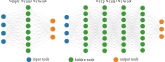
\includegraphics[width=6.5in]{../figures/simple_neural_network_vs_deep_learning.jpg}
			\caption{simple neural network vs deep learning}
			\label{fig:simple_neural_network_vs_deep_learning}
		\end{figure}

\pagebreak
	\begin{data}

		Imagenet in 2012 represented a significant step forward in machine learning by introducing the first practical example of deep learning, famously known as AlexNet (Figure~\ref{fig:imageNet_classificatoin_paper}) This model, developed by Geoffrey Hinton and his team, utilized deep convolutional neural networks to dramatically improve the accuracy of image classification, which was a longstanding challenge in the field.


		\begin{figure}[H]
			\centering
			\vspace{-2ex}
			\includegraphics[width=5.0in]{../figures/imageNet_classificatoin_paper}
			\vspace{-4ex}
			\caption{Geoffrey's 2012 paper ``ImageNet Classification with Deep Convolutional Neural Networks''.\protect\footnotemark[1]}
			\label{fig:imageNet_classificatoin_paper}
		\end{figure}
		\footnotetext[1]{Copyright held by Authors and Neural Information Processing Systems Foundation, Inc., used under fair use. $<$https://proceedings.neurips.cc/paper/2012/file/c399862d3b9d6b76c8436e924a68c45b-Paper.pdf$>$}

		The results of AlexNet were rather monumental, reducing the top-5 test error rate to 15.3\% compared to 26.2\% by the next best entry, as shown in Figure~\ref{fig:ImageNet-competition-results}.  This was clear evidence of deep learning's superior capability over traditional machine learning methods, effectively revolutionizing the approach towards machine learning in the broader scientific community.

		\begin{figure}[H]
			\centering
			\includegraphics[width=4.95in]{../figures/ImageNet-competition-results}
			\caption{ImageNet Competition Results showing the impact of deep learning methods on image classification.}
			\label{fig:ImageNet-competition-results}
		\end{figure}

		The implications of this leap forward led to broad applications of deep learning that permeate numerous aspects of technology and science today. The impact of AlexNet and subsequent deep learning developments culminated in the awarding of the 2024 Nobel Prize in Physics to Geoffrey Hinton, recognizing his contributions to the field of artificial neural networks. Figure~\ref{fig:Nobel} shows the 2024 Nobel Award Ceremony in Stockholm Sweden with John Hopfield and Geoffrey Hinton receiving their awards from the King of Sweden. 

		\begin{figure}[H]
			\centering
			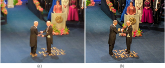
\includegraphics[width=4.95in]{../figures/Nobel}
			\caption{The 2024 Nobel Prize in Physics ``for foundational discoveries and inventions that enable machine learning with artificial neural networks'' was awarded to: (a) John Hopfield and (b) Geoffrey  Hinton. \protect\footnotemark[1]}
			\label{fig:Nobel}
		\end{figure}
		\footnotetext[1]{The author of this text was lucky enough to attend the 2024 Nobel Prize Ceremony in Stockholm and took these pictures.}

	\end{data}


	\subsection{Definition of Machine Learning}

	The definitions and conventions that follow provide a common language and point of reference for all subsequent material:

		\begin{itemize}
			\item	Machine learning is the discipline of creating computer programs that improve automatically by analyzing data. Here a broader and a more engineering-focused definition of Machine learning is provided5:
			\begin{itemize}
				\item {[Machine Learning is the]} field of study that gives computers the ability to learn without being explicitly programmed. Arthur Samuel, 1959.
				\item A computer program is said to learn from experience E with respect to some task T and some performance measure P, if its performance on T, as measured by P, improves with experience E. Tom Mitchell, 1997.
			\end{itemize}
			\item The use of $X$ and $Y$ for variables. 
			\begin{itemize}
				\item For the $i^{\text{th}}$ sample, $x^{(i)}$ contains all its input features (excluding the target), while $y^{(i)}$ denotes the corresponding target value.
				\item General definition:	``Machine learning algorithms are described as learning a target function ($f$) that best maps input variables ($X$) to an output variable ($Y$).''
			\end{itemize}
		\end{itemize}
		
		\begin{equation}
			Y = f(X)
		\end{equation}
		
		\noindent This is described as a standard learning challenge where the goal is to predict future values $Y$ using new samples of input variables $X$. The function $f$ that relates inputs to outputs is not known. If it were, direct application would be possible, eliminating the necessity for learning it via machine learning methods. This process is more complex than it may initially seem. Furthermore, there is an error $e$ associated with this task that is independent of the input data $X$.

	
		\begin{equation}
			Y = f(X) + e
		\end{equation}
		
		\noindent This yields two primary phases in the machine-learning workflow:
		\begin{itemize}
			\item Training: Creating the model is a compute-intensive process often run in a data center
			\item Inference: Using the model can be computationally cheap and even performed ``at the edge''
		\end{itemize}

\pagebreak

			\begin{figure}[t]
				\centering
				\includegraphics[width=\linewidth]{../figures/Supervised_and_unsupervised_machine_learning.png}
				\vspace{-6ex}
				\caption{Supervised vs unsupervised unsupervised machine learning methods\protect\footnotemark[1].}
				\label{fig:Supervised_and_unsupervised_machine_learning}
				\vspace{-1ex}
			\end{figure}

		\footnotetext[1]{modified from: Langs, G., R�hrich, S., Hofmanninger, J. et al., CC BY 4.0 $<$https://creativecommons.org/licenses/by/4.0$>$, via Wikimedia Commons}



	\subsection{Supervision in Machine Learning}
	\vspace{-1ex}

		The general domains of ML can be classified into supervised and unsupervised learning, as shown in figure~\ref{fig:Supervised_and_unsupervised_machine_learning}.

		
		\subsubsection{Supervised Learning}
	\vspace{-1ex}			
			In supervised learning, the data is pre-categorized with labels
			\begin{itemize}[itemsep=0.0ex,topsep=0.0ex]
				\item \textbf{Classification}, The process of categorizing a given set of data into classes
				\item \textbf{Regression}, The process of estimating the relationships between a dependent variables (i.e. output) and one or more independent variables (i.e. input).
			\end{itemize}
			In supervised learning, the training data provided to the algorithm includes the desired solutions, known as labels. A common task within this type of learning is classification. An example of classification is a spam filter, which is trained using numerous emails that are each labeled as either spam or ham. The objective for the spam filter is to learn how to accurately classify new emails based on this training. Regression is another typical task is to predict a target numeric value, such as the price of a house, given a set of features (size, proximity to railroad or highways, age of house, style, etc.) called predictors. To train a system you need to build a model and train in on many house sale examples, including both predictors (house features) and their labels (i.e., prices).
			Some of the most important supervised learning algorithms:
			\begin{itemize}[itemsep=0.0ex,topsep=0.0ex]
				\item	k-Nearest Neighbors
				\item	Linear Regression
				\item	Logistic Regression
				\item	Support Vector Machines (SVMs)
				\item	Decision Trees and Random Forests
				%\item	Neural networks (some)
			\end{itemize}
			
%			\begin{figure}[t]
%				\centering
%				\includegraphics[]{../figures/Ames_simple_linear_regression_model_3}
%				\caption{Estimating the price of a house using the area of its living space.}
%				\label{fig:Boston_simple_linear_regression_model_3}
%			\end{figure}





			
			

			\begin{figure}[H]
				\centering
				\includegraphics[width=4in]{../figures/semantic_word_cloud}
				\caption{A semantic word cloud of Barack Obama's First Inaugural Address \protect\footnotemark[1].}
				\label{fig:data_visualization}
			\end{figure}

		\footnotetext[1]{Modified from: GuoYongzhi, CC BY-SA 4.0 $<$https://creativecommons.org/licenses/by-sa/4.0$>$, via Wikimedia Commons}

			
		\subsubsection{Unsupervised Learning }

In unsupervised learning, the training data is unlabeled, and the system endeavors to learn independently without explicit guidance. For instance, consider a situation where you have extensive data on what people watch on YouTube. You might use a clustering algorithm to identify groups of similar users. However, at no point do you instruct the algorithm on which group a user belongs to; it discovers these connections autonomously. For example, it might identify that the types of videos people watch are closely linked to specific age and income metrics. Older viewers may prefer watching videos about vacations, while younger viewers might watch a lot of educational content, such as Khan Academy.

Visualization algorithms such as that in Figure~\ref{fig:data_visualization}) serve as an important instance of unsupervised learning algorithms: they take in extensive, complex, and unlabeled data and produce a 2D or 3D representation that can be conveniently visualized. These algorithms strive to maintain as much of the original data structure as possible (for example, ensuring that distinct clusters in the input space do not merge in the visual output). This helps in comprehending the organizational structure of the data and potentially uncovering hidden patterns. Other Important concepts in unsupervised learning include
\pagebreak
\begin{itemize}
	\item \textbf{Clustering}, The process of identifying and grouping similar data points in larger datasets without concern for the specific outcome
	\item \textbf{Association}, The process learning a rule-based method for discovering relations between variables data data
	\item \textbf{Dimension Reduction},  The process of reducing the number of input variables in training data.
\end{itemize}
Here are some of the most important unsupervised learning algorithms:
	\begin{itemize}
		\item	Clustering
		\item	k-Means
		\item	Hierarchical Cluster Analysis (HCA)
		\item	Expectation Maximization
	\end{itemize}



%\begin{figure}[H]
%    \centering
%    \includegraphics[width=6.5in]{../figures/iris_species}
%    \caption{Flowers representing three species of iris plants \protect\footnotemark[1]}
%    \label{fig:iris_species}
%\end{figure}
%\footnotetext[1]{Diego Mariano, CC BY-SA 4.0 $<$https://creativecommons.org/licenses/by-sa/4.0$>$, via Wikimedia Commons}


	
	

%		\begin{figure}[H]
%			\centering
%			\includegraphics[width=5.5in]{../figures/Principal_tree_for_Iris_data_set.png}
%			\caption{Principal tree visualization for the Iris data set \protect\footnotemark[1]. }
%			\label{fig:Principal_tree_for_Iris_data_set}
%		\end{figure}
%		\footnotetext[1]{Agor153, CC BY-SA 3.0 $<$https://creativecommons.org/licenses/by-sa/3.0$>$, via Wikimedia Commons}
%


%			\begin{figure}[H]
%				\centering
%				\includegraphics[width=5.5in]{../figures/Softmax_classification.png}
%				\caption{Classification of the three species for the Iris data set.}
%				\label{fig:Softmax_classification}
%			\end{figure}




%\begin{itemize}
%\item	Some important visualization items we will look at in class include. 
%				\begin{itemize}
%					\item	Principal Component Analysis (PCA)
%					\item	Kernel PCA
%					\item	Locally-Linear Embedding (LLE)
%					\item	t-distributed Stochastic Neighbor Embedding (t-SNE)
%				\end{itemize}
%\end{itemize}		

			
			\begin{figure}[H]
			\centering
				\includegraphics[width=6.5in]{../figures/Anomaly_detection}
				\caption{Anomaly Detection for a given set of data.}
				\label{fig:Anomaly_detection}
			\end{figure}
			
Another key application of unsupervised learning is anomaly detection as shown in figure~\ref{fig:Anomaly_detection}. The goal is to flag unusual credit-card transactions that may signal fraud, spot defects on a production line, or filter out outliers before passing a dataset to another learning algorithm. The model is first exposed to many examples of normal behavior so it can build a reference profile. When a new observation arrives it checks how closely the example matches that profile and labels it normal or anomalous accordingly.


		
		\subsubsection{Semisupervised Learning}
			
			Certain algorithms are designed to manage partially labeled training data, typically characterized by a substantial amount of unlabeled data with a minimal amount of labeled data  as shown in figure~\ref{fig:semisupervised_learning}.
			Many semi-supervised learning algorithms are hybrid forms, integrating features of both unsupervised and supervised learning approaches.
			
			An example is seen in image hosting services like Google Photos. Upon uploading your family images, the system automatically recognizes and groups repeated appearances of the same individuals across different photos, such as person 1 in photos A, C, and D and person 2 in photos A, B, and E. This clustering is the unsupervised component of the algorithm. The system then only needs a single label for each person to subsequently identify and tag everyone in all images, enhancing the ease of searching through photos.

			
			
			\begin{figure}[H]
				\centering
				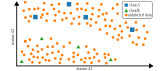
\includegraphics[width=\linewidth]{../figures/semisupervised_learning}
				\caption{Semisupervised learning enabling the use of a limited set of labeled data to infer the labels of larger unlabeled datasets.}
				\label{fig:semisupervised_learning}
			\end{figure}
		
		\subsubsection{Reinforcement Learning}
			
			Reinforcement learning follows a distinct paradigm in which an autonomous agent repeatedly interacts with its environment. At each step the agent observes the current state, chooses and executes an action, and then receives feedback in the form of a reward or penalty; as shown in figure~\ref{fig:reinforcement_learning_control_diagram}. By sampling many such cycles the agent gradually discovers a strategy, known as a policy, that maps perceived situations to actions so as to maximise the total reward accumulated over time.

			
%			\begin{ML_case_study}
%				
%			\textbf{Jean-Baptiste Mouret}
%				
%			\begin{itemize}
%				\item	Teaching creatures to walk
%				\item	\url{https://youtu.be/kQ2bqz3HPJE?t=58}
%				\item	Jean-Baptiste Mouret (2015) has been developing robots that give me nightmares. 
%				\item	The robot learns how to walk by ``searching'' a space to decide how to walk. 
%			\end{itemize}
%				
%			\end{ML_case_study}
%
%			\begin{ML_case_study}
%	
%			\textbf{Walking robots}
%				
%			\begin{itemize}
%				\item	\url{https://youtu.be/T-c17RKh3uE?t=23}
%				\item	It takes about 40 seconds for the robot to re-learn how to walk. It can be 96\% as fast with a broken leg. 
%			\end{itemize}
%						
%		\end{ML_case_study}		

			
			
			\begin{figure}[H]
				\centering
				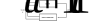
\includegraphics[width=\linewidth]{../figures/reinforcement_learning_control_diagram}
				\caption{Reinforcement learning diagram.}
				\label{fig:reinforcement_learning_control_diagram}
			\end{figure}
			
			

	
	\subsection{Types of learning (Batch and Online)}
		
Machine learning systems can be broadly categorized based on how they process and learn from data.

%\todo{make figures for online and batch learning}


		\subsubsection{Batch Learning}
		
		

In batch learning, the system is fully trained using the entirety of the available data, which often demands significant time and computational resources, and is thus usually performed offline. Initially, the system undergoes training; after which, it is deployed into production where it no longer learns but merely applies the previously acquired knowledge. This method is referred to as offline learning. The deployment phase, known as inference, is typically executed swiftly.

To update a batch learning system with new information, such as recognizing a novel form of spam, it is necessary to develop a completely new version of the system. This version must be trained from the ground up using the entire dataset, both old and new data, before replacing the older system in production.

\begin{figure}[H]
	\centering
	\includegraphics[width=\linewidth]{../figures/training_batch}
	\caption{Batch learning framework with separate training and inference stages. }
	\label{fig:training_batch}
\end{figure}



Despite these challenges, the training, evaluation, and deployment processes of a machine learning system can be automated, allowing even batch learning systems to adapt to changes. This approach is straightforward and usually effective; however, training on a full dataset can be time-consuming - often taking many hours - hence, systems are usually updated no more frequently than daily or weekly. Moreover, utilizing the full dataset requires extensive computing resources, such as CPU power, memory, disk space, and network bandwidth. For organizations with vast amounts of data, the costs of daily retraining from scratch can be prohibitively expensive.

If the dataset is exceptionally large, employing a batch learning algorithm may become impractical. Additionally, in situations where autonomous learning is essential and computational resources are limited, such as with smartphone applications or extraterrestrial rovers, the need to manage large datasets and conduct lengthy training sessions daily poses significant challenges.
		
		
		\subsubsection{Online Learning}


\begin{figure}[H]
	\centering
	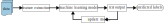
\includegraphics[width=\linewidth]{../figures/training_online}
	\caption{Online learning framework where data is used to continuously training (or update / fine-tune) the model. }
	\label{fig:training_onilne}
\end{figure}

			
Online learning trains a model incrementally by presenting new data points one at a time or in small mini-batches. Each update is computationally light and fast, allowing the model to refresh its knowledge continuously as fresh data streams in. This approach is particularly appropriate for systems that:
\begin{itemize}[itemsep=0.25ex]
    \item receive data continuously, such as stock prices,
    \item need to quickly or autonomously adapt to changes,
    \item have limited computing resources: once an online learning system processes new data instances, they can be discarded to save space, unless there is a need to revert to a previous state and ``replay'' the data.
\end{itemize}
Online learning is also useful for managing large datasets that exceed the memory capacity of a single machine, known as out-of-core learning. The algorithm processes parts of the data, conducts a training step, and repeats this until all the data has been processed.

A critical parameter in online learning systems is the learning rate, which dictates how rapidly the system adapts to changing data. A high learning rate allows for rapid adaptation but may also lead to quick forgetting of old data and training on noise. A low learning rate results in slower learning and reduced sensitivity to variations in new data.

		
		\subsubsection{Bad Data in Machine Learning }
		\vspace{-1ex}		

		A significant challenge in online learning is the system's susceptibility to performance degradation when exposed to poor quality data. This is particularly problematic in live systems where clients might quickly notice issues. For instance, bad data could originate from a malfunctioning robot sensor or an attempt to manipulate search engine rankings through spamming. To mitigate these risks, it is crucial to vigilantly monitor the system and quickly disable learning or revert to a previously effective state if a decline in performance is observed. Additionally, monitoring the input data for anomalies and employing anomaly detection algorithms can help identify and respond to aberrant data.


			\begin{figure}[H]
				\centering
				\includegraphics[width=6in]{../figures/cows}
				\vspace{-1ex}
				\caption{Training a machine learning algorithm to recognize cows may end up just learning to recognize grass. humorously called ``short-cut learning''\protect\footnotemark[1].}
				\label{fig:cows}
			\end{figure}


			\footnotetext[1]{Screen shoot of a Google image search for cows taken by the Austin Downey, all images stated to be under a creative commons license per Google search tools; also assumed to be fair use under given the educational purpose of this text, via \url{https://www.google.com/}}


		For example, imagine training a convolutional neural network to recognize cows (Figure~\ref{fig:cows}). Every image in the training set shows black-and-white cattle standing on lush green pasture, so the easiest statistical cue for the model to latch onto is the dominant green background rather than the animals themselves. At inference time, the network confidently labels any scene filled with grass as ``cow,'' yet fails when presented with a cow on snow or asphalt. In other words, it has learned ``grass recognition,'' not ``cow recognition''.


		
	\subsection{Learning Approaches: Instance-Based and Model-Based}
		

Another method of classifying machine learning systems is based on their generalization capabilities. Typically, the main objective in machine learning is to make predictions, which requires the system to generalize from its training examples to new, unseen instances. Achieving high performance on training data is useful but not the ultimate goal; the system must also excel when confronted with new data.
There are primarily two strategies for generalization: instance-based learning and model-based learning.
		

\begin{figure}[H]
	\centering
	\includegraphics[width=\linewidth]{../figures/instance_based_learning}
	\caption{Instance-based learning where the class of a unknown instance is inferred from the its distance to data points with known labels.}
	\label{fig:instance_based_learning}
\end{figure}
		
		\subsubsection{Instance-based learning}
		

One of the simplest learning strategies is rote memorization. For instance, a spam filter built on this principle would only mark emails as spam if they match previously flagged emails exactly. While this approach is straightforward, it's hardly the most effective.
A more sophisticated spam filter could extend its detection capabilities to include emails that closely resemble known spam messages. This approach necessitates a metric for measuring the similarity between two emails. A basic method might involve counting the shared words between emails. Under this system, an email would be classified as spam if it shares a significant number of words with an email already identified as spam.
This method exemplifies instance-based learning (Figure~\ref{fig:instance_based_learning}), where the system memorizes specific examples and uses a similarity metric to generalize to new instances.
			
			

		\pagebreak
		
		\subsubsection{Model-based learning}
				\vspace{-1ex}
		
Another approach to generalization involves constructing a model based on a set of examples and then using this model to make predictions as shown in figure~\ref{fig:model_based_learning}. This method is known as model-based learning.
			
			
			\begin{figure}[H]
			\centering
				\includegraphics[width=6in]{../figures/model_based_learning}
				\caption{Model-based learning where the class of a unknown instance is inferred from its location in reference to a model trained on the data with known labels.}
				\label{fig:model_based_learning}
			\end{figure}
		
	
			\begin{figure}[H]
			\centering
				\includegraphics[width=6in]{../figures/ml_map}
				\caption{Flowchart of estimators used in the scikit learn library that intends guide users for what algorithms to use for a given case\protect\footnotemark[1].}
				\label{fig:ml_map}
			\end{figure}
			\footnotetext[1]{Scikit-learn algorithms cheat sheet, permissive simplified BSD license and assumed to be fair use under given its nature as documentation and the educational purpose of this text, via \url{https://scikit-learn.org/stable/tutorial/machine_learning_map/index.html}}
	
	
		\subsubsection{Selecting methods:}	


One of the initial challenges faced by newcomers to machine learning is selecting the appropriate algorithms (or estimators) for specific tasks. This is due to the fact that various algorithms excel with different kinds of data and problems. The flowchart depicted in Fig.~\ref{fig:ml_map}, which originates from the scikit-learn library documentation, is intended to guide users in choosing the most suitable algorithms for their particular datasets.


				\vspace{-1ex}
		\subsection{The Unreasonable Effectiveness of Data}
				\vspace{-1ex}

In a landmark study released in 2001, Microsoft researchers Michele Banko and Eric Brill demonstrated that a variety of Machine Learning algorithms, even relatively straightforward ones, achieved similar levels of performance on a complex task of natural language disambiguation when provided with sufficient data. This finding is illustrated in figure~\ref{fig:data_versus_algorithms} and further discussed in their paper\protect\footnotemark[1].

\footnotetext[1]{Michele Banko and Eric Brill. ``Scaling to very very large corpora for natural language disambiguation.'' Proceedings of the 39th annual meeting of the Association for Computational Linguistics. 2001.}

\begin{figure}[H]
\centering
	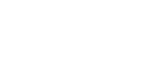
\includegraphics[width=6.5in]{../figures/data_versus_algorithms.png}
	\vspace{-2ex}
	\caption{Learning curves for four algorithms studied in Banko and Brill showing the importance of the amount of data when compared to algorithm selection.  }
	\label{fig:data_versus_algorithms}
\end{figure}


As the authors put it: ``these results suggest that we may want to reconsider the tradeoff between spending time and money on algorithm development versus spending it on corpus development.''. Or put more directly ``The Unreasonable Effectiveness of Data''\protect\footnotemark[2]. It's important to recognize, however, that small and medium-sized datasets remain prevalent, and acquiring additional training data is not always straightforward or economical. Therefore, the significance of algorithm selection should not be overlooked.

\footnotetext[2]{Halevy, Alon, Peter Norvig, and Fernando Pereira. ``The unreasonable effectiveness of data.'' IEEE intelligent systems 24.2 (2009): 8-12.}


\end{document}

